\subsection{L'IA et l'INA}

%% Introduction et présentation des utilisation de l'IA à l'INA %%

L'IA est en train d'avoir un impact profond dans le traitement documentaire des institutions patrimoniales et sur toute la médiation des contenus. A l'INA, outre les projets destinés à améliorer les documents (augmentation de la résolution, restauration d'images, colorisation, doublage synchro-labiale)\footnote{Projets évoqués dans la formation e-learning \enquote{Formation à la data à l'INA} sur \enquote{Le déploiement de l'IA dans le traitements de l'image à des fins de vente}}, les principaux travaux utilisant l'IA sur le traitement documentaires visent à semi-automatiser l'analyse des collections. En passant par l'analyse et la reconnaissance de l'image, des voix et des sons. Différents projets visent à automatiser la segmentation des émissions (délimitation de séquences temporelles d'une émission), la reconnaissance d'entité nommées ainsi que l'indexation automatique, grâce à laquelle il serait possible de générer des résumés et des mots-clés pour les notices des émissions.\footcite[91]{bassaïstéguy2025}. La vitrine de cette utilisation de l'IA à l'INA est le site data.ina.fr\footcite[]{dataina} qui met à contribution l'analyse des transcription, du sons et des images de journaux télévisés et de chaînes d'informations en continu pour proposer des datavisualisations sur certains sujets. Par exemple, le graphique suivant met à contribution l'analyse des transcriptions automatisées par IA et le repérage d'entité nommées pour faire ressortir les personnalités les plus mentionnées des journaux télévisés.
\begin{figure}[H]
	\centering
	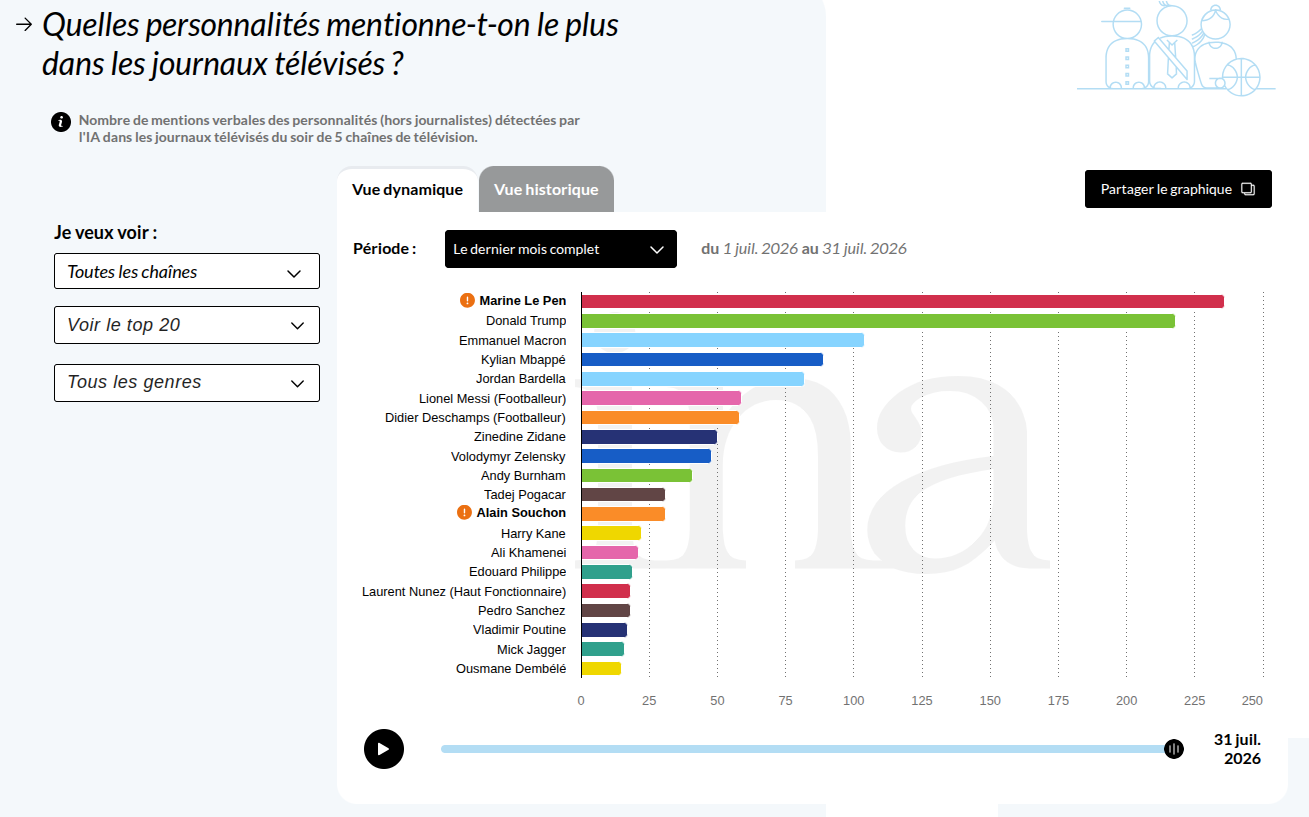
\includegraphics[width=1\linewidth]{./illustrations/dataina.png}
	\caption{Capture d'écran du site data.ina.fr du graphique des personnalités les plus mentionnées dans les journaux télévisés au cours du mois dernier (à la date du 09 septembre 2026).}
	\label{fig:dataina}
\end{figure}
L'existence de ce site manifeste l'aboutissement des travaux sur l'INA sur l'IA et la capacité qu'elle a à se soustraire à une analyse humaine. 

\subsection{l'IA et les documentalistes}

%% Point sur le rôle qu'ont les documentaliste dans l'implantation de l'IA à l'INA et leur avis sur le sujet %%

Si tous ces projets d'utilisation de l'IA ont pour objectif d'améliorer le traitement documentaire d'une façon ou d'une autre, ils ont également un impact sur le cœur même du métier de documentaliste. Si ce sont aux ingénieurs de penser et développer ces outils. C'est aux documentalistes de construire les prompts, de superviser l'apprentissage des outils, et vérifier le travail réalisé et de le corriger. C'est un sujet qui suscite beaucoup d'échanges entre documentalistes : entre la peur de voir disparaître l'essence de son métier et l'assurance de voir de plus en plus de fonds pouvant être décrit et indexé. Ces sentiments se retrouvent auprès des deux documentalistes interrogés. Sont remis en question notamment la légitimité à utiliser de plus en plus d'IA pour des questions de temps et d'argent quand cet outil entraîne également des coûts non négligeables ainsi que des interrogations d'ordre écologiques. Mais aussi le soulagement de ne plus avoir à traiter des sujets considérés ennuyant ou peu stimulants. 

Et d'un autre côté, sont toujours évoqués l'importance de l'expertise du documentaliste. Il ne semble pas y avoir de crainte pour le moment que l'Intelligence Artificielle soit capable de remplacer l'expertise et l’œil de ces documentalistes. Pour mettre en marche ces IA, la médiation humaine reste au centre de cette évolution. De plus notre documentaliste interrogée remet en cause sa fiabilité. Nous avons évoqué à plusieurs reprises que l'erreur humaine imprégnait le traitement documentaire, quel que soit l'institution patrimoniale mais elle est le plus souvent de l'ordre de l'omission ou de la faute de frappe. Ces erreurs mettent en péril leur repérabilité dans la base de données comme nous l'avions vu avec la notice d'\enquote{Images de Turquie} mais elles ne produisent pas de contre-sens comme le ferait une intelligence artificielle qui hallucine. La documentaliste cite dans ce cas une émission indexée par IA lors de tests qui faisait remonter le terme de terrorisme, jamais évoqué dans l'émission. Cette technologie est toujours en cours d'amélioration mais cela questionne la plus-value d'un outil dont les résultats nécessitent la vérification d'un documentaliste. Dans ce cas le gain de temps supposé est remis en question. 

D'autant plus que l'INA tient une posture de référent dans la conservation et communication d'archives audiovisuelles et qu'il n'est pas envisageable de garder des résumés provoquant des contresens pour l'utilisateur\footnote{(Opinions recueillit lors d'entretiens avec une documentaliste de l'INA, Pascal Lebeurier et Arthur Hénaff, voir la section \enquote{L'impact des nouvelles technologies - de l'IA} ~\ref{ann:transcriptions},\nameref{ann:transcriptions}), p.~\pageref{ann:transcriptions}. Pour plus d'informations sur l'impact de l'IA sur le métier de documentaliste le mémoire \enquote{Evolution du métier de documentaliste dans le contexte du déploiement de l'IA à l'INA} par Ghitta Mellah est à paraître.}. 

De la même façon que l'IA entre de plus en plus dans les habitudes de la société, certaines documentalistes ont également recours à l'IA dans leurs pratiques quotidiennes, en dehors des outils mis à leur disposition ou à tester. Des grands noms parmi les intelligences artificielles conversationnelles comme ChaptGPT, Copilot, Claude sont autant utilisées dans le développement des outils de l'INA que chez les documentalistes pour les accompagner dans leurs missions, en les aidant à rédiger, à se corriger etc... Ici aussi les avis divergent, notre documentaliste interrogée dit préférer rédiger en autonomie mais comprend que d'autres collègues puissent y avoir recours. 

\subsection{L'IA et l'accessibilité aux collections}

%% L'impact direct de l'IA dans le traitement documentaire actuellement (Hors documentalistes)%%

Des documentalistes interrogés, ce ne sont pas forcément toutes ces avancées de l'IA qui revenaient le plus mais plutôt la transcription automatique par IA qui utilise la reconnaissance de la parole et des outils d'indexation assistée\footcite[][150]{caporiondo-prost2026}. Cet outil est souligné comme étant une compensation au manque de description de certaines émissions du à la quantité massive de données, certaines typologies comme les fonds régionaux, longtemps négligés\footnote{(Voir entretien d'une documentaliste de l'INA sur l'impact de la politique documentaire sur les données de description ~\ref{ann:transcriptions},\nameref{ann:transcriptions}), p.~\pageref{ann:transcriptions}.}. Ils contribuent à compenser les différences de politique documentaire et de vocabulaire, notamment lors de l'indexation. Dans ce cas, Pascal Lebeurier nous cite une commande traitant du réchauffement climatique. En se fiant à l'indexation, le document le plus ancien était de 77 mais grâce aux transcriptions, les documentalistes ont pû faire ressortir un document de 1950 utilisant déjà le terme de \enquote{réchauffement climatique}. Encore une fois, les données descriptives décrivaient seulement une \enquote{expédition Groenland}. Les transcriptions viennent compléter les descriptions pré-existantes et parfois compenser leurs défauts et ainsi facilitent l'accès à toutes les collections. 

Mais aujourd'hui, et ce malgré le complément important que ces transcriptions apportent aux notices lacunaires, les transcriptions ne sont pas accessibles à tous les publics. C'est principalement les personnes internes à l'INA qui bénéficient de cette avancée et en écoulement, des personnes qui bénéficient des services de recherche de ces documentalistes comme les professionnels de l'audiovisuels. En effet, ces transcriptions ne sont pour le moment accessibles que sur l'outil de consultation Notilus, toujours en développement et inaccessible aux publics. Pourant la demande est forte, notamment au sein du Lab. Mais il est pleinement envisagé de mettre à disposition des publics ces transcriptions dans les outils en développement comme l'ont évoqué Pascal Lebeurier et Arthur Hénaff\footnote{(Voir transcription des entretiens~\ref{ann:transcriptions},\nameref{ann:transcriptions}), p.~\pageref{ann:transcriptions}.}. 

%% Conclusion %%

L'intégration des transcription par IA est une transformation importante des méthodes de recherche qui permettent de contrebalancer certaines difficultés à la recherche dans les bases de données dues à l'évolution des politique documentaires et à la massification des données. D'une autre part, cela impacte également la pratique du traitement documentaire, leur implication dans les outils d'intelligence artificielle suppose que les institutions ont une grande responsabilité dans la fiabilité des données, surtout pour des institutions comme l'INA ou la BNF qui ont une posture de référents dans leur domaine. Il est également sensé de questionner l'impact que cela aura sur le métier de documentaliste. Ce métier tiens une posture d'expert des collections mais il court de risque de glisser vers une statut de contrôleur des données générées par IA. Nous sommes au cœur d'une évolution majeure des politiques documentaires. Avec l'intelligence artificielle s'ouvre la possibilité d'améliorer l'accessibilité aux collections. Bien qu'elle vienne également avec son lot de nouvelles réflexions. Outre les interrogations sur l'impact écologiques et économiques de telles pratiques ainsi que sur la gouvernance des données, elles portent sur la place de l'expertise des documentalistes mais aussi sur la place à donner à des analyses réalisées par IA dans les notices descriptives. Questionnant au passage la posture de référence que tiennent ces institutions en terme de documentation si la description vient à être totalement automatisée. 